\documentclass[10pt, a4paper]{article}
\usepackage[paper=a4paper, left=1.5cm, right=1.5cm, bottom=1.5cm, top=3.5cm]{geometry}
\usepackage[T1]{fontenc}
\usepackage[spanish]{babel}
\usepackage[utf8]{inputenc}
\usepackage{indentfirst}
\usepackage{fancyhdr}
\usepackage{a4wide}
\usepackage[dvipsnames,usenames]{color}
\usepackage{float}
\usepackage{amsmath}
\usepackage{listings}
\usepackage{listingsutf8}
\usepackage{graphicx}
\usepackage{amsfonts}
\usepackage{verbatim}
\usepackage{latexsym}
\usepackage{lastpage}
\usepackage[colorlinks=true, linkcolor=blue]{hyperref}
\usepackage{calc}

\newcommand{\f}[1]{\text{#1}}
\newcommand{\real}{\mathbb{R}}
\newcommand{\nat}{\mathbb{N}}
\newcommand{\eme}{\mathcal{M}}
\newcommand{\emeh}{\widehat{\mathcal{M}}}
\newcommand{\ere}{\mathcal{R}}

\sloppy

\setlength{\voffset}{-0.5cm}
\setlength{\hoffset}{0.7cm}
\setlength{\headsep}{0pt}
\setlength{\headheight}{0pt}
\setlength{\oddsidemargin}{-0.7in}
\setlength{\marginparwidth}{-0.5cm}
\setlength{\textwidth}{18cm}
\setlength{\footskip}{2pt}
\setlength{\topmargin}{0in}
\setlength{\textheight}{25cm}
\setlength{\fboxrule}{3pt}

\begin{document}
\thispagestyle{empty}
\begin{center}

\Huge{ \bf{UNIVERSIDAD DE BUENOS AIRES}}
\\
\LARGE{\bf{Facultad de Ciencias Exactas y Naturales}}
\\
\textbf{Departamento de Computaci\'on}
\\
\textbf{M\'etodos Num\'ericos}
\vspace{2.0\baselineskip}
\end{center}


\begin{figure}[h] %[h] Aqui [b] para button [t] para top
\begin{center}

\includegraphics[width=100pt]{./image.jpeg}
\end{center}
\end{figure}
\begin{center}
\vspace*{0.7cm}

\huge{\bf TRABAJO PR\'ACTICO N\'UMERO 1}\\
\huge{Efectividad de m\'etodos num\'ericos para hallar ceros de funciones.}
\vspace*{2.2cm}

\end{center}

\LARGE {\textbf{Alumnos:}}\\
\Large{\textsl{Izcovich, Sabrina} $|$ sizcovich@gmail.com}\\
\Large{\textsl{Otero, Fernando} \hspace{0.1cm}$|$ fergabot@gmail.com}\\
\Large{\textsl{Vita, Sebasti\'an} \hspace{0.37cm}$|$ sebastian\_vita@yahoo.com.ar}
\vspace{0.6cm}

\LARGE {\textbf{Palabras Clave:}}\\
\large {Newton - Secante - Bisecci\'on - Estimaci\'on}
\vspace*{1.1cm}

\LARGE{\textbf{Resumen:}}\\
\large {Este trabajo consiste en un an\'alisis de m\'etodos num\'ericos utilizados para hallar ceros de funciones. El objetivo del an\'alisis es estimar los par\'ametros necesarios de una funci\'on D$\Gamma$G para estudiar datos de manera certera y eficiente. Para realizar nuestra experimentaci\'on, incluimos la utilizaci\'on de los M\'etodos de Bisecci\'on, Newton y Secante. Luego de diversas pruebas en las que combinamos distintos paquetes de datos, criterios de parada y m\'argenes de error, hemos concluido que los m\'etodos num\'ericos son muy acertados siempre y cuando los par\'ametros sean los correctos para su buen funcionamiento.}
\newline
 
\newpage
%Pagina de titulo e indice
\thispagestyle{empty}

\tableofcontents

\newpage

\section{Introducci\'on te\'orica}

A lo largo del trabajo pr\'actico, hemos experimentado con distintas herramientas necesarias para obtener resultados precisos que nos permitieran sacar conclusiones significativas y s\'olidas. Este tipo de herramientas consistieron, generalmente, en m\'etodos num\'ericos, f\'ormulas de muestreo probabil\'istico y datos aleatorios. En esta secci\'on, enunciaremos los utensilios utilizados. 
\begin{itemize}
\item \textbf{M\'etodo de Newton:} Esta t\'ecnica num\'erica para resolver un problema de b\'usqueda de ra\'ices f(x) = 0 es una de las m\'as poderosas y conocidas pues permite lograr una convergencia m\'as r\'apida (cuadr\'atica) que la que ofrecen otros tipos de iteraci\'on funcional. Dicho m\'etodo, basado en los polinomios de Taylor, genera la sucesi\'on ${P_{n}}$ definida por $P_{n}$ = $P_{n-1}$ - $\frac{f(P_{n-1})}{f'(P_{n-1})}$, para n $\leq$ 1.

\item \textbf{M\'etodo de Bisecci\'on:} Este m\'etodo consiste en hallar un intervalo [a,b] en el que la funci\'on f resulte continua y f(a).f(b)<0. Basado en el teorema del valor intermedio, la idea del mismo es realizar una b\'usqueda binaria para hallar el punto p perteneciente a (a,b) en el que f(p)=0. Su convergencia est\'a asegurada y la misma es lineal.

\item \textbf{M\'etodo de Secante:} El m\'etodo de secante altera el m\'etodo de Newton aproximando la derivada de la funci\'on afectada utilizando la idea del teorema del valor medio. De esta manera, no resulta necesaria una derivada de la funci\'on. Esto \'ultimo afecta a la convergencia que resulta superlineal en dicho m\'etodo.

\item \textbf{Criterios de parada:} Los criterios de parada utilizados fueron los siguientes (para bisecci\'on, se remplazaron $X_{n}$ por b, $X_{n-1}$ por a y f($X_{n}$) por c):
\begin{itemize}
  \item$|X_{n} - X_{n-1}|$ < $\epsilon$
  \item$\frac{|X_{n} - X_{n-1}|}{|X_{n-1}|}$ < $\epsilon$
  \item$|f(X_{n})|$ < $\epsilon$
  \item$|f(X_{n}) - f(X_{n-1})|$ < $\epsilon$
  \item$\frac{|f(X_{n}) - f(X_{n-1})|}{|f(X_{n-1})|}$ < $\epsilon$
\end{itemize}

\item \textbf{Cambio de base de exponenciales:}\newline
\vspace*{0.3cm}
\centerline{$y = a^x \Leftrightarrow y = e^{mx}$ (con $y = (e^m)^x$).}
 \centerline{Luego, $a = e^m \Leftrightarrow ln(a) = ln(e^m) \Leftrightarrow ln(a) = mln(e)$.}
  \centerline{Como $ln(e) = 1$, queda $ln(a) = m \Rightarrow
  \left\lbrace
  \begin{array}{l}
     \text{si a > 1} \Rightarrow \text{m > 0} \\
     \text{si 0 < a < 1} \Rightarrow \text{m < 0} \\
  \end{array}
  \right.$}

\end{itemize}
\section{Desarrollo}

\large{\textbf{An\'alisis previo:}}

El objetivo del trabajo pr\'actico es hallar las combinaciones de m\'etodos num\'ericos de mayor eficiencia que, junto con los par\'ametros m\'as acordes, otorguen los resultado m\'as cercanos posibles a $\beta$ dado un paquete de datos determinado. Para cumplir con dicho objetivo, utilizamos los m\'etodos:

\begin{itemize}

\item Newton: El uso de este m\'etodo era requerido por la c\'atedra. Dicho m\'etodo tiene su importancia en la convergencia cuadr\'atica ya que es la mejor entre los m\'etodos analizados en clase. Sin embargo, dicha convergencia no est\'a garantizada por un teorema de convergencia global como podr\'ia estarlo el m\'etodo de bisecci\'on. Por lo tanto, es necesario partir de una aproximaci\'on inicial pr\'oxima a la ra\'iz buscada para que el m\'etodo converja debidamente. Este m\'etodo resulta muy interesante pero a la vez muy costoso dado que requiere de la derivada de la funci\'on a utilizar, que en nuestro caso result\'o ser compleja.

\item Secante: Debido a que la convergencia de secante es superlineal, elegimos el m\'etodo para comparar el tiempo de ejecuci\'on del mismo con el de los dem\'as. Por otro lado, nos pareci\'o interesante observar el margen de error que mantiene con Newton al aproximar la derivada con el Polinomio de Taylor para lograr obtener resultados relevantes y encontrar una justificaci\'on para ellos. 

\item Bisecci\'on: Utilizamos este m\'etodo dado que nos result\'o importante asegurarse convergencia en todo momento a pesar de que \'esta sea lineal. Tambi\'en, lo utilizamos para aproximar, tanto el $P_{0}$ en Newton, como el $P_{0}$ y $P_{1}$ en Secante.
\end{itemize}

El procedimiento de nuestro trabajo pr\'actico fue el siguiente:\newline

Elegimos, en primer lugar, la funci\'on que nos result\'o m\'as valorable para analizar. \'Esta result\'o ser la $(5)$ debido a que no contiene la funci\'on $log$, por lo tanto, se deben realizar menos operaciones para resolverla. \'Esto logra que se acarree menos error y nos otorga mayor precisi\'on en los resultados.\newline

En segundo lugar, pensamos en analizar matem\'aticamente la funci\'on con el fin de simplificarla lo m\'aximo posible. Al realizar esto, nos encontramos con que toda conclusi\'on posible depend\'ia del paquete de datos ingresado por lo que el an\'alisis de funci\'on resultaba in\'util. Al simplificar de diversas maneras las funciones utilizadas, los m\'argenes de error hallados eran despreciables. Por ejemplo, estudiamos la diferencia entre los valores de $\eme$ y $\emeh$ calculados por la computadora y simplificando la multiplicaci\'on y divisi\'on por $n$ manualmente. Si bien el resultado de dicha experimentaci\'on demostr\'o una leve mejor\'ia en la cantidad de iteraciones y el error final, decidimos no utilizarlo dado que \'este no resultaba demasiado significante por lo que preferimos evitar posibles confusiones durante la implementaci\'on.\newline

Luego, procedimos a derivar la funci\'on con sus par\'ametros correspondientes:\newline

Nuestra funci\'on:

$$\frac{\eme(2\beta)}{\eme^2(\beta)} = 1 + \beta(\ere(\beta)-\ere(0)) \Leftrightarrow 0 = 1 + \beta(\ere(\beta)-\ere(0)) - \frac{\eme(2\beta)}{\eme^2(\beta)}$$

donde 
$$\eme(s) =  \frac{1}{n}\sum_{i=1}^n{x_i^s}\,, \qquad \emeh(s) = \frac{1}{n}\sum_{i=1}^n{x_i^s \log(x_i)}\,,  \qquad \ere(s) = \frac{\emeh(s)}{\eme(s)}$$

Al derivar t\'ermino a t\'ermino, se obtuvo:

$$\eme'(s) = \frac{1}{n}\sum_{i=1}^n{x_i^s \log(x_i)} \,, \qquad \emeh'(s) = \frac{1}{n}\sum_{i=1}^n{x_i^s \log(x_i)^2}\,,  \qquad \ere'(s) = \frac{\emeh'(s)}{\eme'(s)}$$

Por lo tanto, la derivada result\'o ser:

$$\ere(\beta) + \beta(\ere'(\beta)) - \ere(0) - \frac{2\eme'(2\beta)\eme^2(\beta) - 2\eme(2\beta)\eme(\beta)\eme'(\beta)}{\eme^4(\beta)}$$
\\

\large{\textbf{Implementaci\'on:}}
El paso siguiente consistió en programar en C++ los m\'etodos utilizados, la funci\'on junto con su derivada y el programa para realizar pruebas dado un paquete de datos ingresado. Al implementar las f\'ormulas, utilizamos el cambio de base de funciones exponenciales (explicado en la \textit{Introducci\'on te\'orica}) para simplificarlas. \newline
Nos decidimos por el uso de una lista para manipular las muestras dado que, en otro caso, se hubiese necesitado conocer el tamaño de la muestra (como por ejemplo para usar un vector) y no utilizamos ninguna operaci\'on que una lista no pudiera resolver.
 \newline 
El $main.cpp$ consisti\'o en un men\'u necesario para almacenar los datos que ser\'ian, m\'as tarde, utilizados por las funciones para resolver los m\'etodos. Para realizarlo, nos limitamos a utilizar herramientas conocidas (if, while, etc.) y $printf$'s.\newline
En $formulas.cpp$, escribimos las f\'ormulas utilizadas a lo largo del trabajo pr\'actico. Tanto la funci\'on principal para hallar $\beta$ y su derivada como las funciones que definen a $\tilde{\lambda}$ y $\tilde{\sigma}$ se hallan en este archivo. Para que dichas f\'ormulas fueran legibles, utilizamos las funciones $\eme$, $\emeh$ y $\ere$ para realizar las operaciones necesarias y luego terminar por unirlas correctamente. \newline
En $metodos.cpp$ implementamos los m\'etodos utilizados para hallar los ceros de funci\'on. \'Estos est\'an programados de manera tal a recibir los par\'ametros ingresados por el men\'u principal y realizar las operaciones necesarias a partir de ellos. Para calcular el tiempo de ejecuci\'on de cada prueba experimental introdujimos un clock en milisegundos. Utilizamos, tambi\'en, un switch para calcular el error experimental.\newline

Una vez encontrado $\tilde{\beta}$, \'este es reemplazado en las funciones que fuimos despejando de la siguiente manera para hallar $\tilde{\sigma}$ y $\tilde{\lambda}$:

\begin{eqnarray*}
\tilde{\sigma} & = & \left(\frac{\sum_{i=1}^n{x_i^{\tilde{\beta}}}}{n \tilde{\lambda}} \right)^{1/\tilde{\beta}}\\
\tilde{\lambda} & = &\left[ \tilde{\beta} \left( \frac{\sum_{i=1}^n{x_i^{\tilde{\beta}} \log x_i}}{\sum_{i=1}^n{x_i^{\tilde{\beta}}}} - \frac{\sum_{i=1}^n{\log x_i}}{n} \right)\right]^{-1}\\ 
{}& = & \tilde{\beta}^{-1} \left( \frac{\sum_{i=1}^n{x_i^{\tilde{\beta}} \log x_i}}{\sum_{i=1}^n{x_i^{\tilde{\beta}}}} - \frac{\sum_{i=1}^n{\log x_i}}{n}\right)^{-1}\\
{}& = & \tilde{\beta}^{-1} \left( \frac{n\sum_{i=1}^n{x_i^{\tilde{\beta}} \log x_i} - {\sum_{i=1}^n{x_i^{\tilde{\beta}}}}\sum_{i=1}^n\log x_i}{{n\sum_{i=1}^n{x_i^{\tilde{\beta}}}}}\right)^{-1}\\
{}& = & \frac{1}{\tilde{\beta}} \left( \frac{{n\sum_{i=1}^n{x_i^{\tilde{\beta}}}}}{n\sum_{i=1}^n{x_i^{\tilde{\beta}} \log x_i} - {\sum_{i=1}^n{x_i^{\tilde{\beta}}}}\sum_{i=1}^n\log x_i}\right)\\
{}& = & \left( \frac{{n\sum_{i=1}^n{x_i^{\tilde{\beta}}}}}{\tilde{\beta} n\sum_{i=1}^n{x_i^{\tilde{\beta}} \log x_i} - {\tilde{\beta}\sum_{i=1}^n{x_i^{\tilde{\beta}}}}\sum_{i=1}^n\log x_i}\right)\\
 0 & = & \frac{\tilde{\beta}}{n} \sum_{i=1}^n{\log x_i} - \log {\sum_{i=1}^n{x_i^{\tilde{\beta}}}} + \log(n \tilde{\lambda}) - \psi(\tilde{\lambda})
\end{eqnarray*}
donde $\tilde{\Theta}=(\tilde{\sigma},\tilde{\beta},\tilde{\lambda})$\\

\large{\textbf{Problemas hallados:}}
Al realizar dicho programa nos encontramos con distintas complicaciones: nuestra mayor complicaci\'on result\'o ser que, si bien encontr\'abamos una buena aproximaci\'on de $\beta$, $\tilde{\lambda}$ y $\tilde{\sigma}$ resultaban desacertadas del valor original.\newline 
Luego de distintas pruebas y un an\'alisis exhaustivo, nos percatamos de que la funci\'on $\tilde{\lambda}$ pod\'ia ser reescrita de manera tal que quedara eliminado todo tipo de potencias y se lograra la m\'inima cantidad de operaciones posibles para su resoluci\'on (vistas m\'as arriba). Del mismo modo, para poder realizar ciertos c\'alculos no permitidos en variables de tipo $TFloat$ (como por ejemplo potencia), deb\'iamos pasar la variable a $double$ y luego nuevamente a $TFloat$ dentro de las f\'ormulas mismas. Al tener que realizar este cambio de tipo en numerosas iteraciones, se arrastraba una gran cantidad de error que derivaba en la obtenci\'on de resultados imprecisos. Para resolver esto \'ultimo, decidimos utilizar la funci\'on $exponencial$ definida en $TFloat.h$. De esta manera, no resultaba necesario el cambio de tipo por lo que los valores devueltos resultaban m\'as certeros. Por lo tanto, evitamos los errores de casteo que hac\'ian diferir el valor original con la estimaci\'on en un 300$\%$. Por ejemplo, en vez de encontrar $\lambda$ = 3, encontr\'abamos $\lambda$ = 0,08. Luego de los cambios realizados, la precisi\'on pas\'o a ser del 85$\%$ aproximadamente.\newline

\large{\textbf{Modo de uso del programa:}} 
Nuestro programa corre en Windows 7 y Ubuntu. Para compilarlo, recomendamos usar g++. Para ejecutarlo es necesario compilar $formulas.cpp$, $metodos.cpp$, $TFloat.cpp$ y, por \'ultimo, $main.cpp$. Luego, se debe abrir el ejecutable del main.\newline Una vez abierta la interfaz del programa, se deben completar paso a paso los datos pedidos por \'este necesarios para su funcionamiento. Entre los par\'ametros requeridos se necesitan la precisi\'on de la mantisa, el tipo de error que se desee utilizar (ver criterios de parada en  \textit{Introducci\'on te\'orica}), el m\'aximo error aceptado, la cantidad m\'axima de iteraciones que el programa debe realizar (conocido como ``criterio de parada pesimista``) y, finalmente, el M\'etodo que se desee utilizar (entre Bisecci\'on, Newton y Secante).\newline En el caso de elegir el m\'etodo de Newton, se debe seleccionar entre insertar manualmente un $p_{0}$ o que \'este sea aproximado por el M\'etodo de Bisecci\'on. En el caso en el que el m\'etodo Secante sea el escogido, se deben ingresar los valores $p_{0}$ y $p_{1}$. Por \'ultimo, al elegir el M\'etodo de Bisecci\'on, se requiere determinar un valor positivo y uno negativo para que \'este pueda hallar el cero que se encuentra entre esos dos valores. En el caso en el que el valor ingresado como positivo o negativo no posea dicho signo, \'este volver\'a a ser pedido. Al finalizar, el programa otorgar\'a los valores de $\tilde{\lambda}$, $\tilde{\beta}$ y $\tilde{\sigma}$ como tambi\'en el tiempo que tard\'o en hallar $\tilde{\beta}$, las iteraciones realizadas y el error final.\newline

\large{\textbf{Recuperaci\'on de resultados:}} Para verificar la correctitud de nuestro programa utilizamos los paquetes de datos otorgados por la c\'atedra cuyos par\'ametros eran conocidos. De esta manera, corroboramos los algoritmos realizados y descartamos experimentos innecesarios. Al realizar varias iteraciones llegamos a la conclusi\'on de que los resultados de nuestro programa resultaban satisfactorios para la mayor\'ia de las pruebas realizadas.\newline
 A partir de ese entonces, comenzamos a evaluar resultados de manera organizada variando los par\'ametros paulatinamente. Completamos una planilla en la que congelamos todos los par\'ametros salvo uno. Por ejemplo, evaluamos tres mantisas distintas (t=51, t=25 y t=15 en la mayor\'ia de los casos) para cada m\'etodo utilizando como error m\'aximo 0,0000000001, 500 iteraciones, $x\_2\_62\_35.txt$ como muestra, un $p_{0}$ y un $p_{1}$ determinados. Realizamos lo mismo cambiando los tipos de error, $p_{0}$ y $p_{1}$ para poder incializar las conclusiones de efectividad. De estas pruebas retuvimos los par\'ametros a estimar, la duraci\'on de la ejecuci\'on del programa, la cantidad de iteraciones realizadas por el mismo y el error final obtenido para cada una de ellas. A partir de esto, obtuvimos los resultados expuestos posteriormente.

\section{Resultados}

Decidimos presentar los resultados con gr\'aficos de histogramas dado que es una herramienta muy simple a la hora de analizarlos y \'estos pueden ser vistos de manera clara. Para ello, utilizamos $Matlab$ aplicando las funciones otorgadas por la c\'atedra ($dibujarHistyAjuste.m$, $GGDpdf\_c.m$ y $leer\_datos.m$).\newline
Los tests fueron realizados con los archivos $x_2\_62\_35.txt$, $x\_15\_9\_3.txt$ y $ X1.txt$. Utilizamos como mantisa los valores del conjunto t={15,18,25,40,51} y los criterios de parada enunciados en la \textit{Introducci\'on te\'orica}. Como error m\'aximo permitido, utilizamos los valos de $\epsilon$ = {2.88e-005, 1e-10, 0.001, 0.5}. Por \'ultimo, las cantidades m\'aximas de iteraciones evaluadas fueron 4000, 2000 y 500.\newline

Los resultados obtenidos fueron los siguientes:\newline

Analicemos, en primer lugar, el siguiente conjunto de datos:

\begin{figure}[H]
\begin{center}
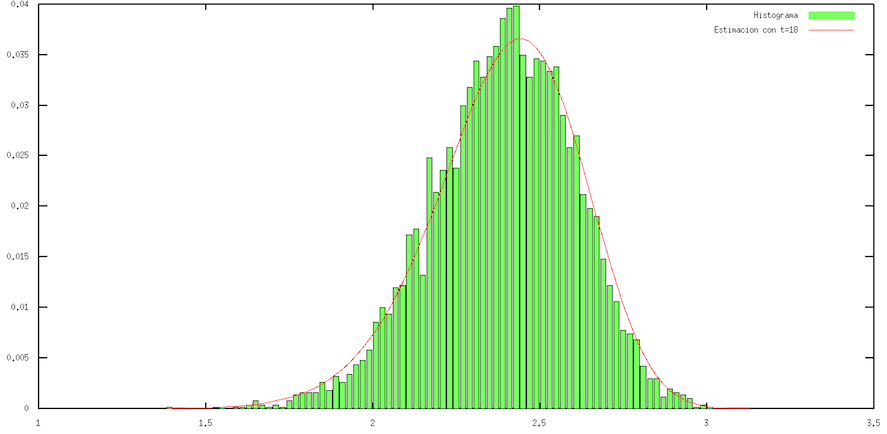
\includegraphics[width=370pt]{./Biseccion_18.png}
\caption[h]{Estimaci\'on del paquete de datos x\_2\_62\_35 con Bisecci\'on}{Precisi\'on t = 18}
\end{center}
\end{figure}

\begin{figure}[H] %[h] Aqui [b] para button [t] para top
\begin{center}
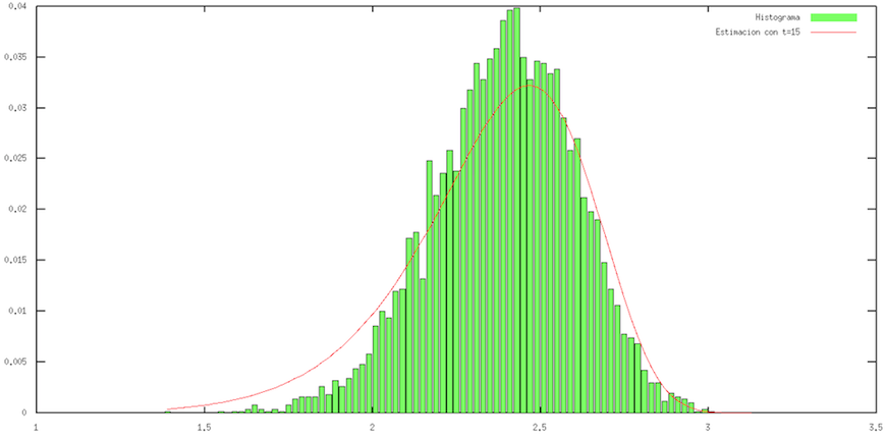
\includegraphics[width=370pt]{./Newton_15.png}
\caption[h]{Estimaci\'on del paquete de datos x\_2\_62\_35 con Newton}{Precisi\'on t = 15}
\end{center}
\end{figure}

\begin{figure}[H] %[h] Aqui [b] para button [t] para top
\begin{center}
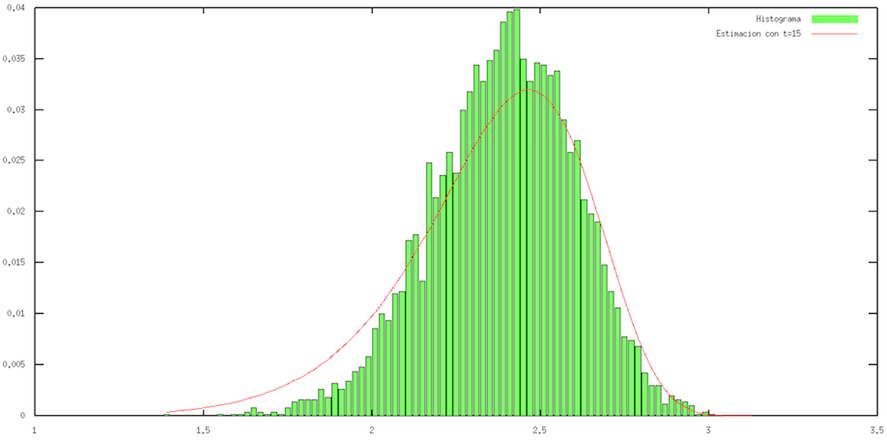
\includegraphics[width=370pt]{./Secante_15.png}
\caption[h]{Estimaci\'on del paquete de datos x\_2\_62\_35 con Secante}{Precisi\'on t = 15}
\end{center}
\end{figure}

En estos gr\'aficos se evaluaron los tres m\'etodos con lo siguiente:
\begin{itemize}
\item Mantisa: 15 para Newton y Secante, 18 para Bisecci\'on
\item Criterio de parada: $|f(X_{n})|$ < $\epsilon$ 
\item Error m\'aximo aceptable: 0.0000000001
\item M\'axima cantidad de iteraciones: 500
\item Muestra evaluada: x\_2\_62\_35.txt
\end{itemize}

\large{\textbf{Resultados observados:}} En el caso del M\'etodo de Bisecci\'on, podemos observar que la curva de estimaci\'on supera el valor de 0.035 (siendo 0.04 el m\'aximo valor del histograma) por lo que se asemeja considerablemente al histograma de datos. Por otro lado, la curva de estimaci\'on del M\'etodo de Newton no alcanza el valor 0.035 sino que su m\'aximo se mantiene en un valor cercano a 0.032. Dicha curva se encuentra ligeramente desfasada a la derecha en comparaci\'on con el histograma. Por \'ultimo, la curva de estimaci\'on del M\'etodo de Secante posee su m\'aximo en el valor 0.0325. Esta curva se encuentra tambi\'en sutilmente desfasada hacia la derecha de acuerdo al histograma de datos.\newline

\begin{figure}[H]
\begin{center}
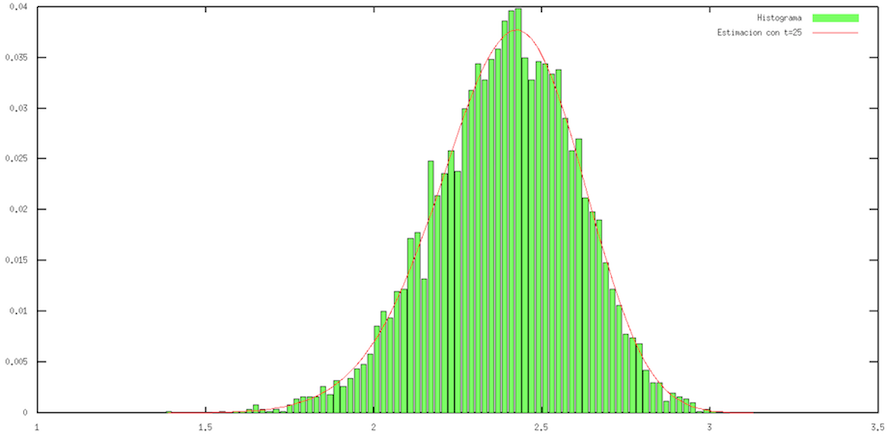
\includegraphics[width=370pt]{./Biseccion_25.png}
\caption[h]{Estimaci\'on del paquete de datos x\_2\_62\_35 con Bisecci\'on}{Precisi\'on t = 25}
\end{center}
\end{figure}

\begin{figure}[H] %[h] Aqui [b] para button [t] para top
\begin{center}
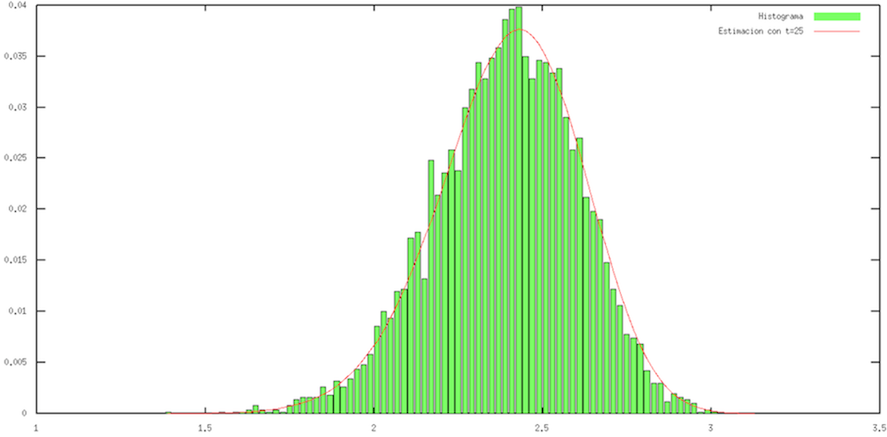
\includegraphics[width=370pt]{./Newton_25.png}
\caption[h]{Estimaci\'on del paquete de datos x\_2\_62\_35 con Newton}{Precisi\'on t = 25}
\end{center}
\end{figure}

\begin{figure}[H] %[h] Aqui [b] para button [t] para top
\begin{center}
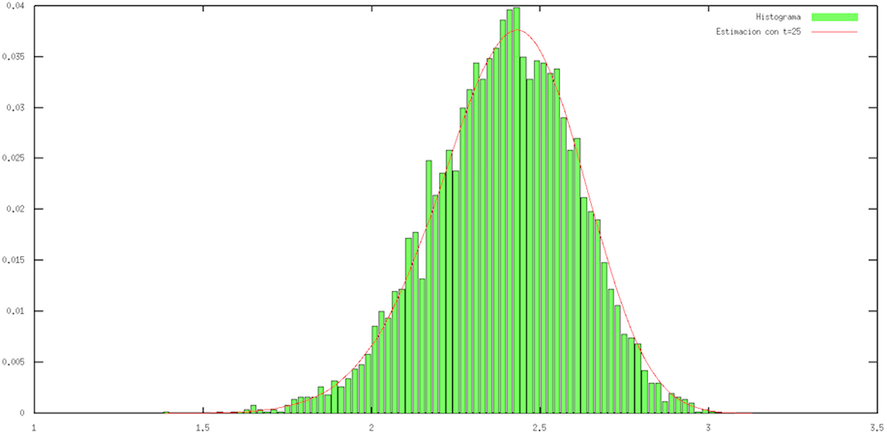
\includegraphics[width=370pt]{./Secante_25.png}
\caption[h]{Estimaci\'on del paquete de datos x\_2\_62\_35 con Secante}{Precisi\'on t = 25}
\end{center}
\end{figure}

En estos gr\'aficos se evaluaron los tres m\'etodos con lo siguiente:
\begin{itemize}
\item Mantisa: 25
\item Criterio de parada: $|f(X_{n})|$ < $\epsilon$ 
\item Error m\'aximo aceptable: 0.0000000001
\item M\'axima cantidad de iteraciones: 500
\item Muestra evaluada: x\_2\_62\_35.txt
\end{itemize}

\large{\textbf{Resultados observados:}} En primer lugar, podemos observar que el m\'aximo alcanzado por la curva de estimaci\'on del M\'etodo de Bisecci\'on supera el valor de 0.035 alcanzando casi a 0.038. Esta curva se mantiene semejante al histograma de datos en todo su alcance. Luego, podemos ver que en el caso del M\'etodo de Newton, el m\'aximo valor alcanzado es cercano al 0.038. Del mismo modo, la curva se mantiene semejante al histograma en todo su alcance, marcando una leve cercan\'ia del lado izquierdo a los valores del interior del histograma. Por \'ultimo, en el M\'etodo de Secante podemos ver que el m\'aximo alcanzado por la curva es de 0.038. La curva permanece similar al histograma de datos en toda su longitud.\newline

\begin{figure}[H] %[h] Aqui [b] para button [t] para top
\begin{center}
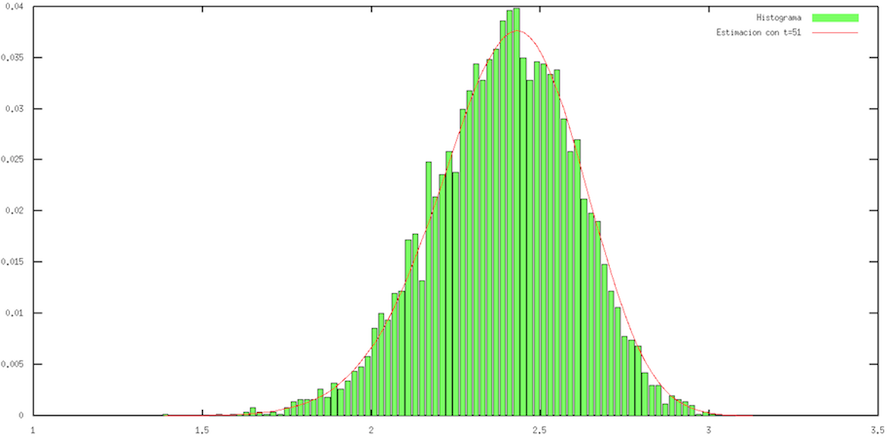
\includegraphics[width=370pt]{./Biseccion_51.png}
\caption[h]{Estimaci\'on del paquete de datos x\_2\_62\_35 con Bisecci\'on}{Precisi\'on t = 51}
\end{center}
\end{figure}

\begin{figure}[H] %[h] Aqui [b] para button [t] para top
\begin{center}
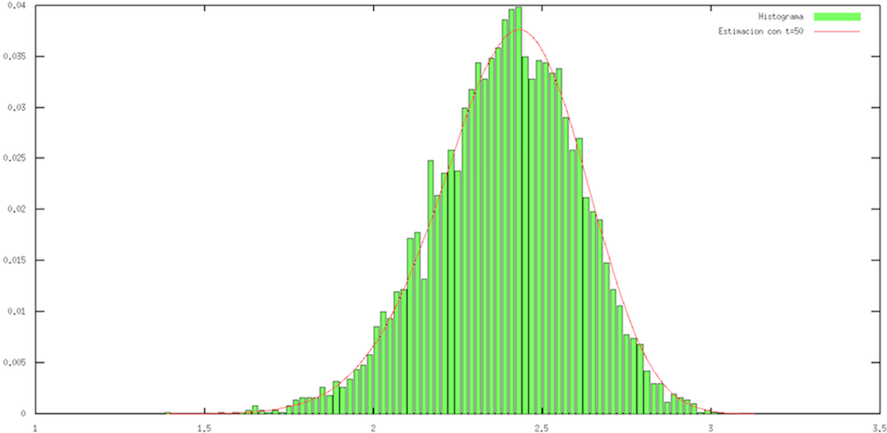
\includegraphics[width=370pt]{./Newton_50.png}
\caption[h]{Estimaci\'on del paquete de datos x\_2\_62\_35 con Newton}{Precisi\'on t = 50}
\end{center}
\end{figure}

\begin{figure}[H] %[h] Aqui [b] para button [t] para top
\begin{center}
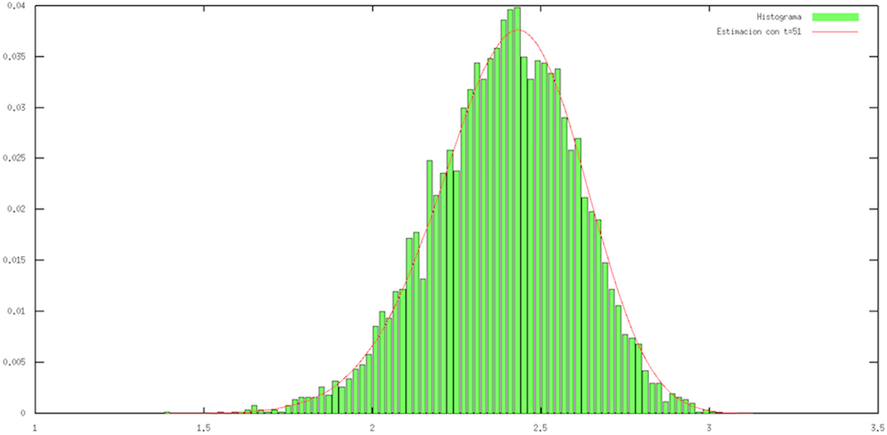
\includegraphics[width=370pt]{./Secante_51.png}
\caption[h]{Estimaci\'on del paquete de datos x\_2\_62\_35 con Secante}{Precisi\'on t = 51}
\end{center}
\end{figure}

En estos gr\'aficos se evaluaron los tres m\'etodos con lo siguiente:
\begin{itemize}
\item Mantisa: 51 para Bisecci\'on y Secante, 50 para Newton
\item Criterio de parada: $|f(X_{n})|$ < $\epsilon$ 
\item Error m\'aximo aceptable: 0.0000000001
\item M\'axima cantidad de iteraciones: 500
\item Muestra evaluada: x\_2\_62\_35.txt
\end{itemize}

\large{\textbf{Resultados observados:}} En primer lugar, podemos observar que el m\'aximo alcanzado por la curva de estimaci\'on del M\'etodo de Bisecci\'on es 0.038. Esta curva se mantiene semejante al histograma de datos en todo su alcance. Luego, podemos ver que en el caso del M\'etodo de Newton, el m\'aximo valor alcanzado es cercano al 0.038. Del mismo modo, a curva se mantiene semejante al histograma en todo su alcance. Por \'ultimo, en el M\'etodo de Secante podemos ver que el m\'aximo alcanzado por la curva es de 0.038. La curva permanece similar al histograma de datos en toda su longitud.\newline

Otros resultados obtenidos fueron los siguientes:
\begin{itemize}
\item Al probar los m\'etodos con una precisi\'on menor a 15, los resultados obtenidos fueron Nan en la gran mayor\'ia de los casos.
\item Al variar los criterios de parada, los resultados se mantuvieron muy semejantes al criterio de parada analizado anteriormente.
\end{itemize}
\section{Discusi\'on}

Para lograr relativizar los resultados, decidimos crear gr\'aficos comparativos en los que se estudiaran \'unicamente esos par\'ametros. Para ello, tomamos 3 datos de nuestra muesta (uno con precisi\'on t = 18, uno con t = 25 y otro con t = 51). Dichos gr\'aficos resultaron ser los siguientes:\newline

\large{\textbf{Comparaci\'on de la cantidad de iteraciones respecto de la precisi\'on de la mantisa.}}\newline

\begin{figure}[H] %[h] Aqui [b] para button [t] para top
\begin{center}
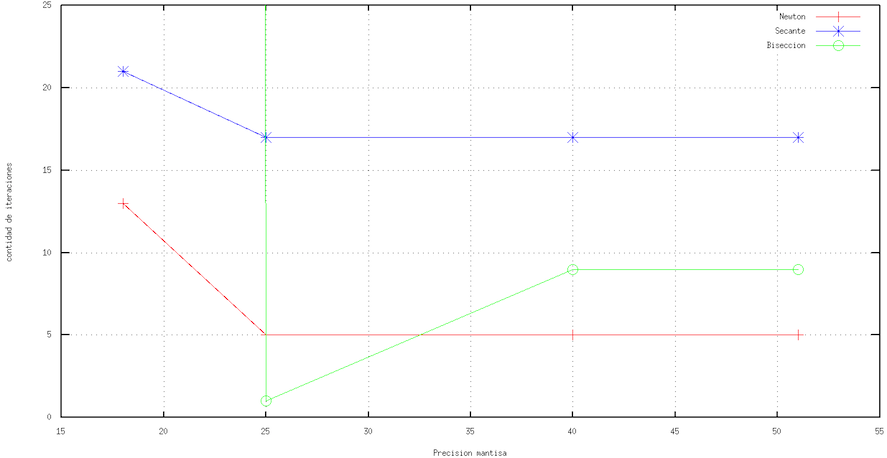
\includegraphics[width=370pt]{./cantidaditeraciones_mantisa.png}
\caption[h]{Comparaci\'on de la cantidad de iteraciones con respecto a la precisi\'on de la mantisa.}{Paquete de datos x\_2\_62\_35.txt}
\end{center}
\end{figure}

\begin{itemize}
\item Error m\'aximo aceptable: 0.0000288
\item Criterio de parada: $|f(X_{n})|$ < $\epsilon$ 
\item $p_{0}$ en Newton: 10
\item $p_{0}$ en Secante: 10
\item $p_{1}$ en Secante: 11
\item Intervalo en Bisecci\'on: [10,3]
\item M\'axima cantidad de iteraciones: 4000
\item Muestra evaluada: x\_2\_62\_35.txt
\end{itemize}

\large{\textbf{Observaciones:}}
En esta figura se compara la cantidad de iteraciones con respecto a la precisi\'on de la mantisa del paquete de datos x\_2\_62\_35 con un error de 0.0000288.\newline
Podemos observar que, tanto en el M\'etodo de Newton como en el de Secante, la cantidad de iteraciones se mantiene relativamente constante entre una precisi\'on de 50 y 25 (en 5 para Newton y en 17 para Secante). Luego, dicho valor disminuye en Secante (pasando a valer 21 siendo 18 la precisi\'on) y aumenta en Newton (pasando a ser 13 iteraciones en 18 de mantisa). Por otro lado, podemos ver que el M\'etodo de Bisecci\'on se mantiene constante en 9 iteraciones hasta 40 de mantisa. Luego, una vez que la precisi\'on pasa a valer 25, dicho valor desciende a 1 para alcanzar las 4000 iteraciones en 18 de precisi\'on. Esto \'ultimo no es del todo claro en nuestra figura dado que debimos recortarla para que fueran claros los dem\'as valores alcanzados por las curvas.


\begin{figure}[H] %[h] Aqui [b] para button [t] para top
\begin{center}
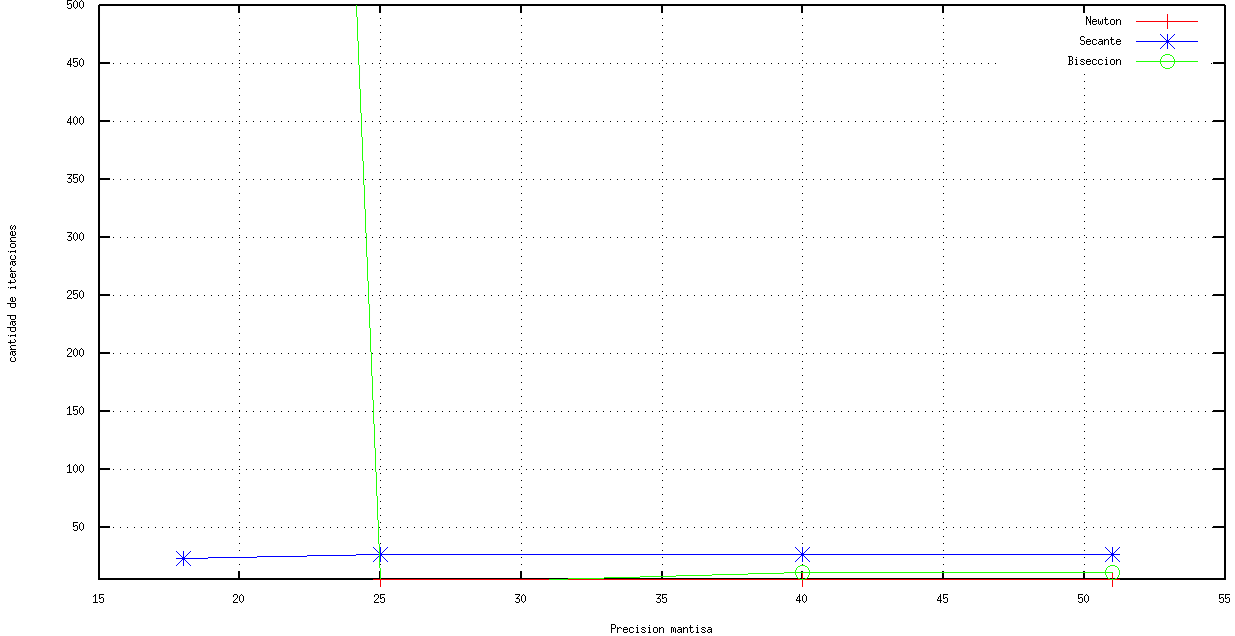
\includegraphics[width=370pt]{./cantidaditeraciones_mantisaerror.png}
\caption[h]{Comparaci\'on de la cantidad de iteraciones con respecto a la precisi\'on de la mantisa.}{Paquete de datos x\_2\_62\_35.txt - Error 0.000001}
\end{center}
\end{figure}

\begin{itemize}
\item Error m\'aximo aceptable: 0.000001
\item Criterio de parada: $|f(X_{n})|$ < $\epsilon$ 
\item $p_{0}$ en Newton: 10
\item $p_{0}$ en Secante: 10
\item $p_{1}$ en Secante: 11
\item Intervalo en Bisecci\'on: [10,3]
\item M\'axima cantidad de iteraciones: 4000
\item Muestra evaluada: x\_2\_62\_35.txt
\end{itemize}

\large{\textbf{Observaciones:}}
En esta figura se compara la cantidad de iteraciones con respecto a la precisi\'on de la mantisa del paquete de datos x\_2\_62\_35 con un error de 0.000001.\newline
Si bien en nuestro gr\'afico el m\'aximo valor mostrado en la cantidad de iteraciones es 1000, \'este deber\'ia ser, en realidad, 4000. Dado que la escala deb\'ia quedar proporcional para que los dem\'as m\'etodos pudieran ser reconocidos gr\'aficamente, decidimos recortarlo. Podemos observar que el M\'etodo de Bisecci\'on se mantiene en una cantidad de 11 iteraciones en 51 de precisi\'on para luego bajar a 1 en 25 y finalizar por remontar a las 4000 iteraciones en 18. Por otro lado, al pasar de 25 a 51 de mantisa, la cantidad de iteraciones se mantiene constante en 5 en el M\'etodo de Newton. Al pasar de 25 a 18 de precisi\'on, la cantidad de iteraciones de dicho m\'etodo pasa a 4000. Del mismo modo, entre 51 y 18 de precisi\'on, podemos ver que el M\'etodo Secante se mantiene en una cantidad de 27 iteraciones.


\begin{figure}[H] %[h] Aqui [b] para button [t] para top
\begin{center}
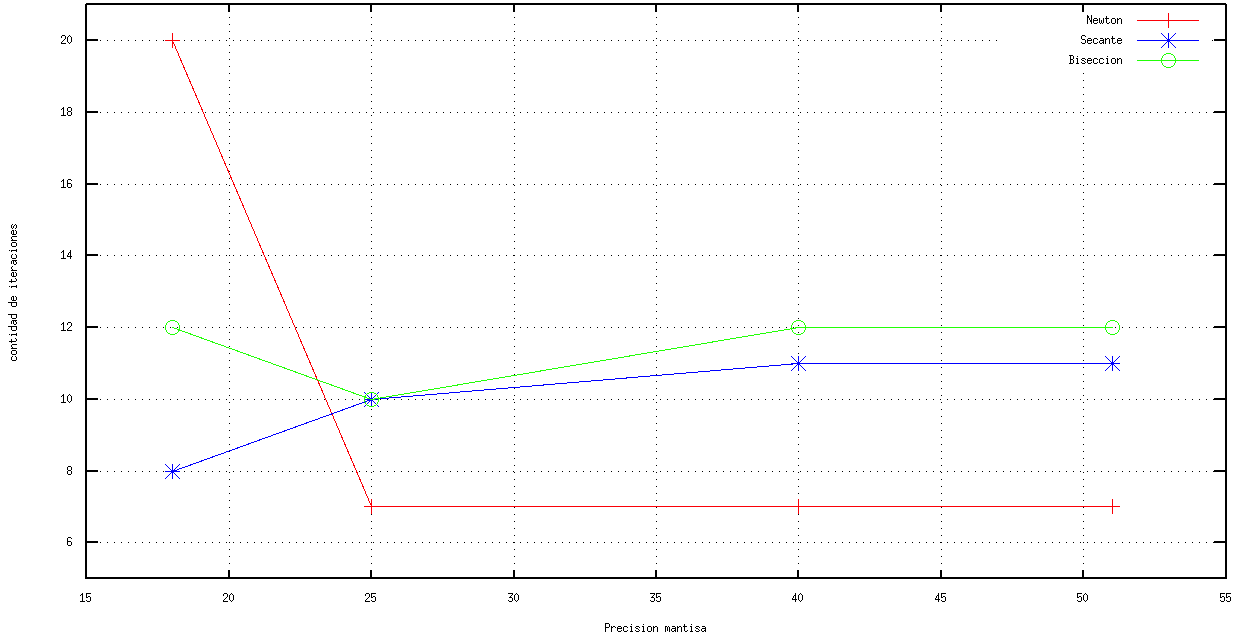
\includegraphics[width=370pt]{./cantidaditeraciones_mantisax1.png}
\caption[h]{Comparaci\'on de la cantidad de iteraciones con respecto a la precisi\'on de la mantisa.}{Paquete de datos X1.txt}
\end{center}
\end{figure}

\begin{itemize}
\item Error m\'aximo aceptable: 0.0000288
\item Criterio de parada: $|f(X_{n})|$ < $\epsilon$ 
\item $p_{0}$ en Newton: 10
\item $p_{0}$ en Secante: 10
\item $p_{1}$ en Secante: 11
\item Intervalo en Bisecci\'on: [10,3]
\item M\'axima cantidad de iteraciones: 4000
\item Muestra evaluada: X1.txt
\end{itemize}

\large{\textbf{Observaciones:}}
En este gr\'afico se compara la cantidad de iteraciones con respecto a la precisi\'on de la mantisa del paquete de datos X1 con un error de 0.0000288.\newline
Podemos percibir que el M\'etodo de Newton mantiene la cantidad de iteraciones firme en 7 entre una precisi\'on de 25 y 51 de mantisa. Luego, al disminuir la precisi\'on a 18, pasa a 20 iteraciones. Por otra parte, el M\'etodo de Secante se mantiene en 11 iteraciones entre 51 y 40 para luego disminuirlas a 10 hasta 25 de precisi\'on y volver a bajarlas a 8. Finalmente, el M\'etodo de Bisecci\'on se mantiene constante en 12 iteraciones hasta alcanzar el valor de 40 de precisi\'on, para disminuirlas a 10 iteraciones en 25 y terminar incrementandolas 12 nuevamente con 18 de mantisa.\newline

\begin{figure}[H] %[h] Aqui [b] para button [t] para top
\begin{center}
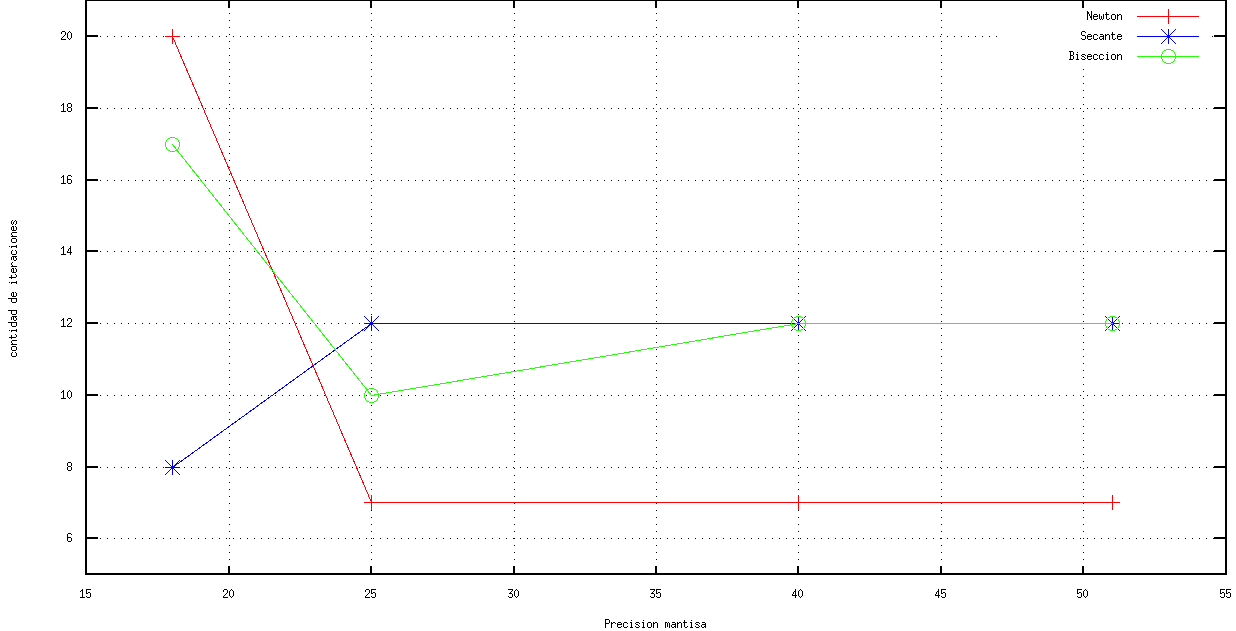
\includegraphics[width=370pt]{./cantidaditeraciones_mantisax1error.png}
\caption[h]{Comparaci\'on de la cantidad de iteraciones con respecto a la precisi\'on de la mantisa.}{Paquete de datos X1.txt - Error de 0.000001}
\end{center}
\end{figure}

\begin{itemize}
\item Error m\'aximo aceptable: 0.000001
\item Criterio de parada: $|f(X_{n})|$ < $\epsilon$ 
\item $p_{0}$ en Newton: 10
\item $p_{0}$ en Secante: 10
\item $p_{1}$ en Secante: 11
\item Intervalo en Bisecci\'on: [10,3]
\item M\'axima cantidad de iteraciones: 4000
\item Muestra evaluada: X1.txt
\end{itemize}

\large{\textbf{Observaciones:}}
En esta figura, se compara la cantidad de iteraciones con respecto a la precisi\'on de la mantisa del paquete de datos X1 con el error 0.000001.\newline
Podemos observar que el M\'etodo de Newton mantiene constante la cantidad de iteraciones (en 7) entre una precisi\'on de 51 y 25 . Luego, al disminuir la precisi\'on, dicho valor disminuye a 20. En el caso de Secante, la cantidad de iteraciones se mantiene en 12 hasta una precisi\'on de 25 para luego disminuir este valor llegando a las 8 iteraciones en 18 de mantisa. Por otro lado, el M\'etodo de Bisecci\'on se mantiene constante en 12 iteraciones hasta llegar a 40 de precisi\'on para luego descender a 10 en 25 de precisi\'on y elevarse nuevamente a 17 una vez que la mantisa alcanza un valor de 18.\newline
 
 
\large{\textbf{An\'alisis sobre las observaciones:}}\newline
A partir de las observaciones realizadas previamente, podemos señalar que al alcanzar un valor de precisi\'on menor a 25, la cantidad de iteraciones se eleva (como en Newton y Bisecci\'on). En cuanto la precisi\'on a alcanzar es demasiado alta, dicha subida se vuelve excesiva al punto de hacer divergir gran parte de las experimentaciones. Por este motivo, nos result\'o imprescindible el uso de una cota superior para la cantidad de iteraciones a realizar por el programa dado que, en el caso contrario, el programa podr\'ia haber alcanzado un bucle infinito.\newline

En el caso de Secante, se puede visualizar de forma clara que en la mayor\'ia de los casos y siempre que la precisi\'on fuera pequeña, la cantidad de iteraciones suele disminuir y no divergir, por lo que alcanza el error buscado.

Por otro lado, se puede notar que cuando la precisión varía entre 51 y 25, la cantidad de iteraciones se mantiene constante fluctuando muy levemente en algunos casos (como por ejemplo Newton en la Figura 10). Analizando todos los tests realizados, pudimos observar que el M\'etodo de Newton es el que menos iteraciones realiza, sigui\'endolo el M\'etodo de Bisecci\'on para terminar por el M\'etodo de Secante.\newline

\large{\textbf{An\'alisis de errores:}}
\begin{figure}[H] %[h] Aqui [b] para button [t] para top
\begin{center}
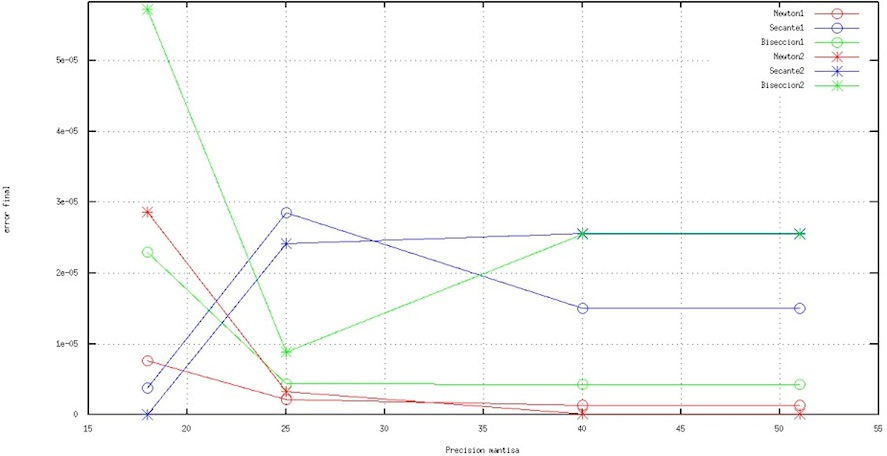
\includegraphics[width=370pt]{./error1.jpg}
\caption[h]{Comparaci\'on del error final con respecto a la precisi\'on de la mantisa.}{Criterio de parada: $|f(X_{n})|$ < $\epsilon$}
\end{center}
\end{figure}

\begin{itemize}
\item Criterio de parada: $|f(X_{n})|$ < $\epsilon$ 
\item M\'axima cantidad de iteraciones: 4000
\item Error m\'aximo aceptable: 0.0000288
\item Secante1 - Newton1 - Bisecci\'on1: Corresponden a la muestra X1.txt
\item Secante2 - Newton2 - Bisecci\'on2: Corresponden a la muestra x\_2\_62\_35.txt
\end{itemize}


\begin{figure}[H] %[h] Aqui [b] para button [t] para top
\begin{center}
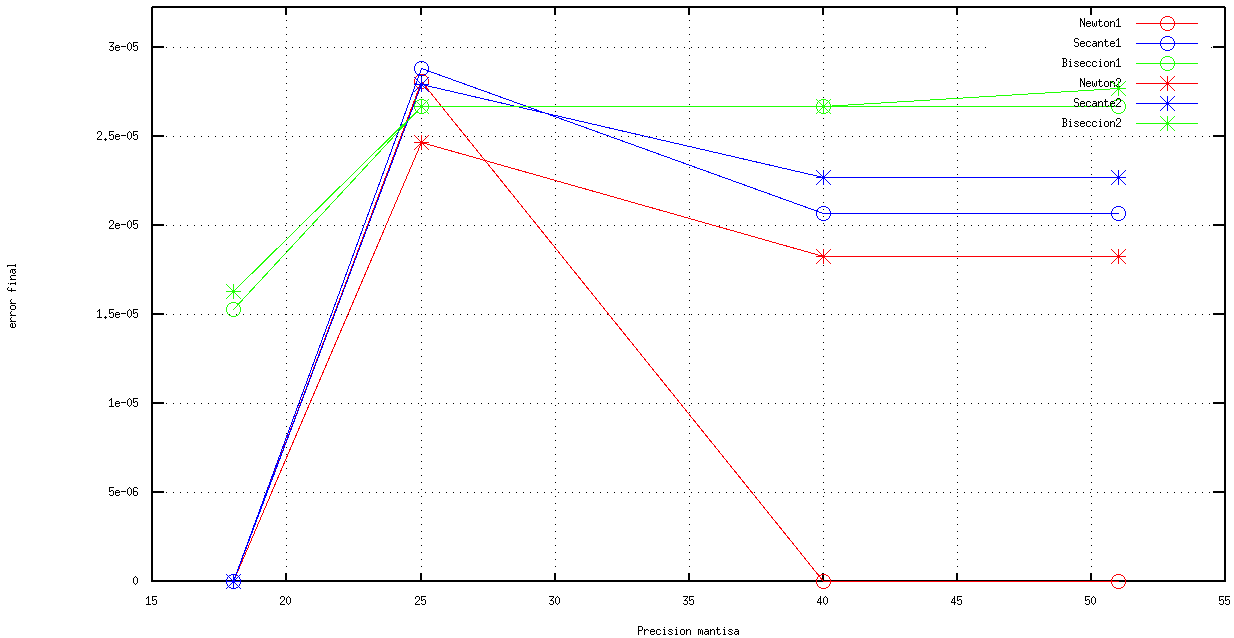
\includegraphics[width=370pt]{./error2.png}
\caption[h]{Comparaci\'on del error final con respecto a la precisi\'on de la mantisa.}{Criterio de parada: $|f(X_{n}) - f(X_{n-1})|$ < $\epsilon$}
\end{center}
\end{figure}

\begin{itemize}
\item Criterio de parada: $|f(X_{n}) - f(X_{n-1})|$ < $\epsilon$ 
\item M\'axima cantidad de iteraciones: 4000
\item Error m\'aximo aceptable: 0.0000288
\item Secante1 - Newton1 - Bisecci\'on1: Corresponden a la muestra X1.txt
\item Secante2 - Newton2 - Bisecci\'on2: Corresponden a la muestra x\_2\_62\_35.txt
\end{itemize}


\begin{figure}[H] %[h] Aqui [b] para button [t] para top
\begin{center}
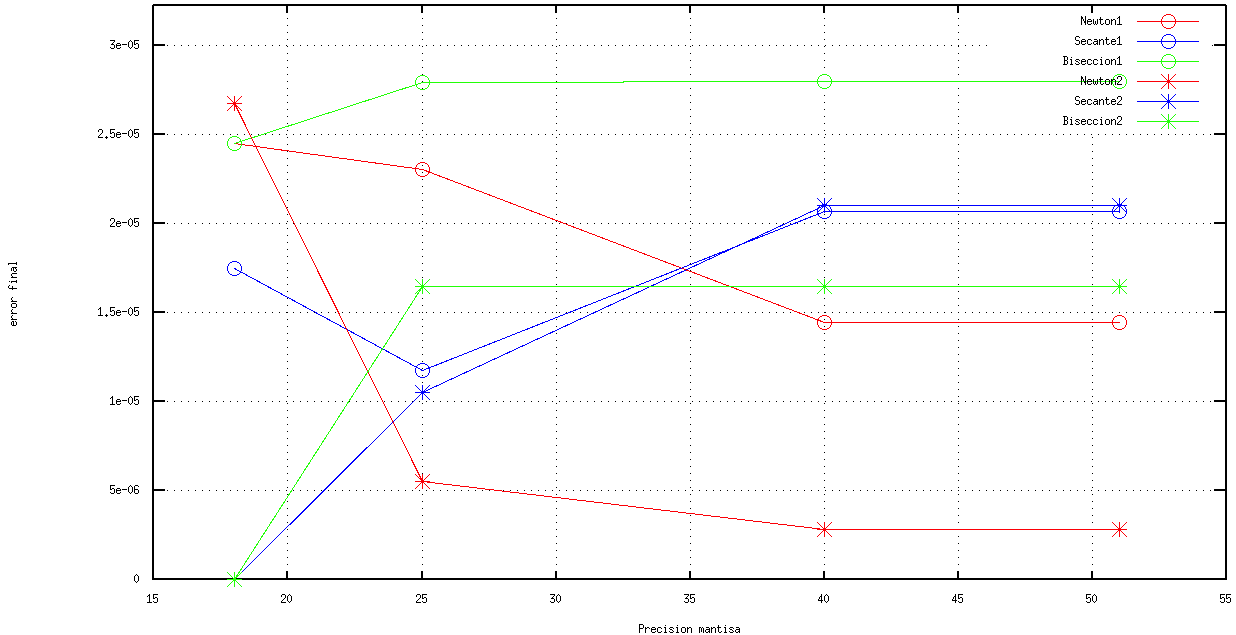
\includegraphics[width=370pt]{./error3.png}
\caption[h]{Comparaci\'on del error final con respecto a la precisi\'on de la mantisa.}{Criterio de parada: $\frac{|X_{n} - X_{n-1}|}{|X_{n-1}|}$ < $\epsilon$}
\end{center}
\end{figure}

\begin{itemize}
\item Criterio de parada: $\frac{|X_{n} - X_{n-1}|}{|X_{n-1}|}$ < $\epsilon$
\item M\'axima cantidad de iteraciones: 4000
\item Error m\'aximo aceptable: 0.0000288
\item Secante1 - Newton1 - Bisecci\'on1: Corresponden a la muestra X1.txt
\item Secante2 - Newton2 - Bisecci\'on2: Corresponden a la muestra x\_2\_62\_35.txt
\end{itemize}



\begin{figure}[H] %[h] Aqui [b] para button [t] para top
\begin{center}
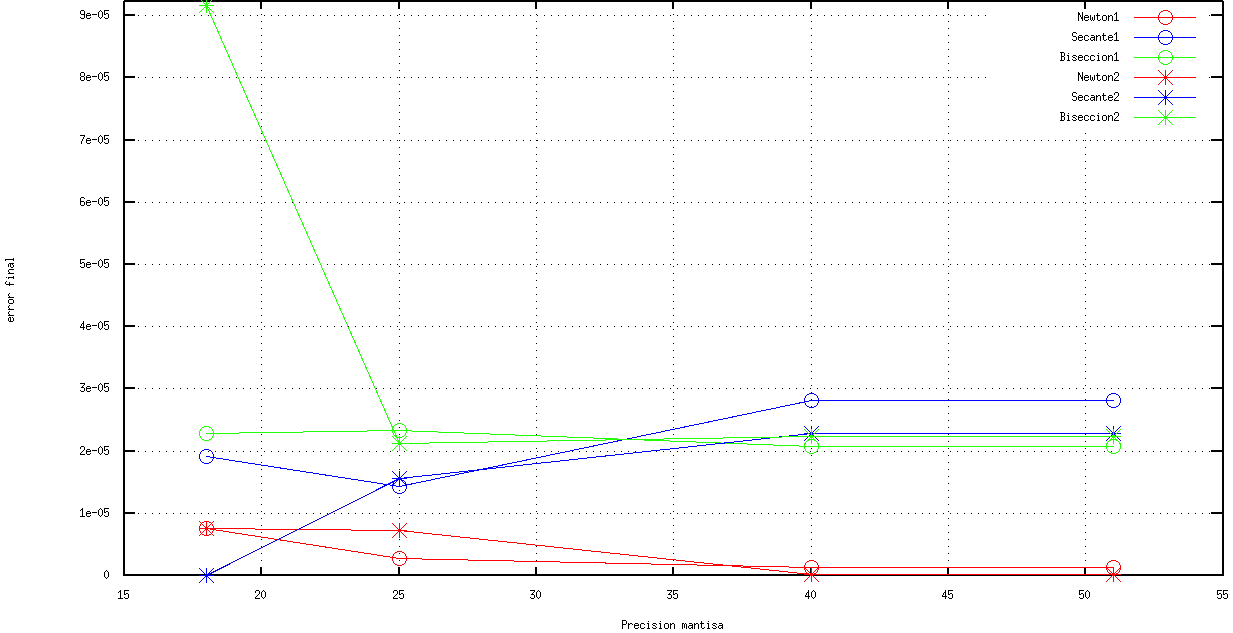
\includegraphics[width=370pt]{./error4.png}
\caption[h]{Comparaci\'on del error final con respecto a la precisi\'on de la mantisa.}{Criterio de parada: $|f(X_{n}) - f(X_{n-1})| < \epsilon$}
\end{center}
\end{figure}

\begin{itemize}
\item Criterio de parada: $|f(X_{n}) - f(X_{n-1})| < \epsilon$
\item M\'axima cantidad de iteraciones: 4000
\item Error m\'aximo aceptable: 0.0000288
\item Secante1 - Newton1 - Bisecci\'on1: Corresponden a la muestra X1.txt
\item Secante2 - Newton2 - Bisecci\'on2: Corresponden a la muestra x\_2\_62\_35.txt
\end{itemize}

\begin{figure}[H] %[h] Aqui [b] para button [t] para top
\begin{center}
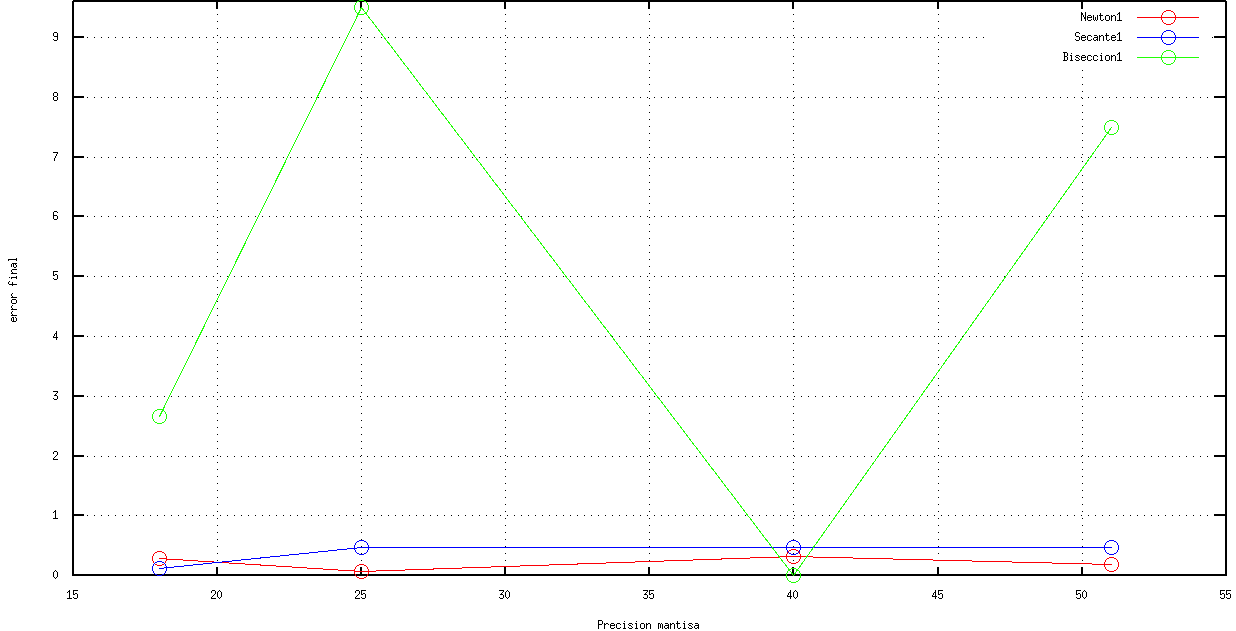
\includegraphics[width=370pt]{./error5.png}
\caption[h]{Comparaci\'on del error final con respecto a la precisi\'on de la mantisa.}{Criterio de parada: $\frac{|f(X_{n}) - f(X_{n-1})|}{|f(X_{n-1})|}$ < $\epsilon$}
\end{center}
\end{figure}

\begin{itemize}
\item Criterio de parada: $\frac{|f(X_{n}) - f(X_{n-1})|}{|f(X_{n-1})|}$ < $\epsilon$
\item M\'axima cantidad de iteraciones: 4000
\item Error m\'aximo aceptable: 0.0000288
\item Secante1 - Newton1 - Bisecci\'on1: Corresponden a la muestra X1.txt
\item Secante2 - Newton2 - Bisecci\'on2: Corresponden a la muestra x\_2\_62\_35.txt
\end{itemize}

\large{\textbf{Observaciones de los gr\'aficos de criterios de parada:}}\newline

En el caso de los 5 criterios de parada, decidimos hacer un an\'alisis general entre ellos ya que no expon\'ian muchas diferencias en cuanto a su esencia. 
Para poder analizarlos correctamente, deber\'iamos realizar una divici\'on en cuanto a la cantidad de precisi\'on a utilizar. Si miramos los valores de t m\'as altos (entre 25 y 50), lo primero que puede ser visto en los criterios es que el M\'etodo de Newton es el que menos error suele tener. Esta caracter\'istica lo beneficia mucho y es la causa por la que suele ser uno de los m\'etodos de mayor convergencia. A continuaci\'on de \'este, se encuentra el M\'etodo Secante y, por \'ultimo, el de Bissecci\'on.\newline
Si analizamos los t's m\'as chicos, el panorama parece ser completamente distinto ya que la regularidad del error que se obtiene con valores altos de t no se obtiene con los bajos. Es por esto que en muchos casos, al ser t muy chico, el error aumenta mucho y esto hace que no se pueda llegar con facilidad a la cota establecida por el error m\'inimo. Por lo tanto, \'este termina resultando del m\'etodo por la cota superior de iteraciones.\newline

\large{\textbf{An\'alisis del tiempo de ejecuci\'on de cada m\'etodo:}}\newline

\begin{figure}[H] %[h] Aqui [b] para button [t] para top
\begin{center}
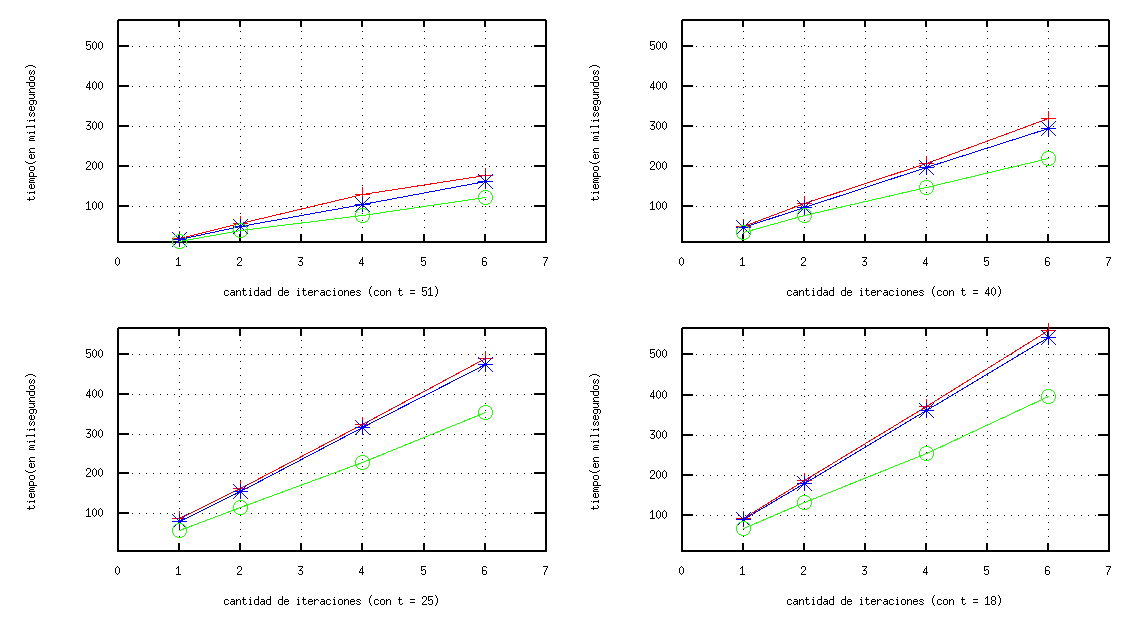
\includegraphics[width=500pt]{./tiempo.png}
\caption[h]{Comparaci\'on del tiempo de ejecuci\'on del programa respecto de la cantidad de iteraciones.}{Pruebas realizadas con t=18, t=25, t=40 y t=51}
\end{center}
\end{figure}

El gr\'afico fue confeccionado con el paquete $x\_2\_62\_35.txt$ utilizando para Newton $p_{0}$=10, para Secante $p_{0}$=11 y $p_{1}$=10 y para Bisecci\'on los extremos 3 y 10. Adem\'as, se realiz\'o con 0.000000001 como error m\'aximo.\newline

En este gr\'afico, se puede observar claramente c\'omo a menor precisi\'on, mayor es la demora al ejecutar las iteraciones. Adem\'as, se puede ver c\'omo cada iteraci\'on realizada por el M\'etodo de Newton tiene mayor retardo que las realizadas por M\'etodo de Secante, que, a su vez, es mayor que las ejecutadas por el M\'etodo de Bisecci\'on.\newline


\large{\textbf{A) Casos particulares:}}
\newline
En la muestra $x\_2\_62\_35$, vimos que el M\'etodo de Bisecci\'on con $|f(X_{n})|$ < $\epsilon$ y 25 iteraciones, resolvi\'o el problema en una \'unica iteraci\'on devolviendo $\tilde{\beta}$=6.5 (siendo $\beta$=6.2) con un error final de 8.82149e-006. Dicho resultado result\'o sorprendente dado a que el valor m\'as pr\'oximo a $\beta$ hallado gracias a estimaciones result\'o ser 6.44. Por lo tanto quedamos perplejos al ver que con una \'unica iteraci\'on se pudiera alcanzar un valor tan pr\'oximo al buscado.\newline

\large{\textbf{B) Variaciones:}}
\newline
No siempre un criterio de parada fue el mejor para un m\'etodo determinado. Las variaciones de la precisi\'on y el $\epsilon$ permitieron hallar las combinaciones m\'as eficientes, diferenciando claramente entre una elecci\'on y otra.\newline

\large{\textbf{C) Resultados parciales:}}
\newline
Se destacan de la muestra la franja de t=[40,52] con pocas variaciones para el ejemplo, la franja t=(40,25] con leves pero mayores variaciones, y la franja t=(25,15) donde los resultados se alejaban sensiblemente de los reales.\newline
Adem\'as de los resultados ($\tilde{\beta}$, $\tilde{\lambda}$ y $\tilde{\sigma}$), las diferentes precisiones modifican sensiblemente los tiempos y las iteraciones. A menor precisi\'on hay más iteraciones y \'estas consumen m\'as tiempo.\newline

Los m\'etodos elegidos para las funciones dadas se comportaron mejor con los criterios de parada 1, 2 y 4. El criterio n\'umero 5 s\'olo nos brind\'o informaci\'on con un error menor a 0.5.\newline

Observando los tiempos y las iteraciones notamos que las iteraciones de Bisecci\'on son mucho m\'as r\'apidas que las de Secante y Newton. Haciendo que poca diferencia entre la cantidad de iteraciones de un m\'etodo y otro d\'e como resultado que Bisecci\'on termine antes su ejecuci\'on.\newline

En cuanto a los errores resultantes al finalizar los m\'etodos, Newton siempre termina m\'as cerca del cero que los otros m\'etodos.\newline

Los resultados obtenidos en cuanto a cantidad de iteraciones realizadas por los métodos es coherente con la teor\'ia: Newton converge m\'as r\'apido que Secante, y \'este que Biseccion.\newline
Tambi\'en encontramos coherentes los resultados de tiempo (por su relaci\'on con la cantidad de iteraciones) y de error, contrastando con la teor\'ia.\newline

Encontramos que para \'esta funci\'on, la forma de parada 5 no nos brindaba informaci\'on (los m\'etodos realizaban en la mayor\'ia de los casos la m\'aximo cantidad de iteraciones).\newline
\'Esta comprobaci\'on se hizo con varios par\'ametros de entrada para cada funci\'on ($\epsilon$ = 1E-10, 1E-6, 0.0001, 0.001, 0.5)\newline
Los test con $\epsilon \leq$ 0.5 no aportaron datos pero los tests con $\epsilon \geq$ 0.001 s\'i. Los datos aportados no son significativos en comparaci\'on con el resto de los datos obtenidos.\newline
Gracias a los \'ultimos tests y al an\'alisis de tError=5, creemos que el inconveniente viene a ra\'iz de que \'este critero de parada da un n\'umero muy chico, y por eso suele no aportar mucha informaci\'on.\newline


\section{Conclusiones}

Hemos concluido que el mejor tiempo de ejecuci\'on result\'o ser el del M\'etodo de Newton que, a su vez, fue el que menos iteraciones realiz\'o para hallar los ceros de funci\'on como tambi\'en el que menos error obtuvo.\newline

 - Con t<40 los valores se comienzan a diferenciar, alej\'andose del $\beta$ real. Con t<=25 se diferencian m\'as r\'apido.\newline
 
 - Con t<=18 se observan algunos errores finales igualados a 0, de lo que concluimos que el n\'umero a representar está fuera de la escala de n\'umeros que se pueden representar con \'esta precisi\'on.\newline

 - Con t< 15 se observan varios (o todos) los valores como Nan.\newline

 - El tError=5 no nos dio datos \'utiles de error ni iteraciones para$ \epsilon$ > 0.5\newline

Hemos encontrado de forma emp\'irica que para una funci\'on a la cual le conocemos la derivada, el M\'etodo de Newton es más eficaz que los métodos Secante y Bisecci\'on. \'Esta eficiencia est\'a determinada por la precisi\'on, la cantidad de iteraciones y el tiempo que le toma al algoritmo resolver el problema dado.

Tambi\'en hemos notado las diferencias entre una precisi\'on y otra y los diferentes criterios de parada. Como las variaciones pod\'ian resultar desde pequeñas variaciones hasta en m\'etodos que no cumpl\'ian su cometido.

Las diferencias de los distintos $\epsilon$ s\'olo dieron resultados interesantes al analizar tError=5, ya que en los otros casos dieron el esperado resultado de, a menor $\epsilon$, menor error y menos iteraciones.

En el caso del criterio de parada Nro 5, entendimos que el criterio es tan riguroso que s\'olo con un $\epsilon$ chico y mucha precisi\'on resulta \'util.

Encontramos un tope a las iteraciones entre 2000 y 4000, para distinguir los m\'etodos que terminaban de los que no. Decidimos mostrar todos los experimentos con 4000 iteraciones máximas para que sean m\'as claros.

Hemos notado que, si bien hay una diferencia sensible entre la cantidad de iteraciones de Newton y las de los otros m\'etodos, entre Bisecci\'on y Secante no siempre es tan notable. Incluso, hubo casos donde Bisecci\'on fue mucho más r\'apido que Secante por el hecho de que cada iteración de Bisecci\'on es más r\'apida que las de Secante.

\section{Ap\'endices}
\subsection{A}
El objetivo del trabajo pr\'actico es implementar un programa que permita estimar los par\'ametros $\Theta=(\sigma,\beta,\lambda)$ a partir de un conjunto de $n$ datos. Para ello, se deber\'a resolver la ecuaciones (5) o (6).
Evaluando los distintos m\'etodos vistos en clase que permitan resolver este problema, se deber\'a realizar una implementaci\'on cumpliendo lo siguiente:
\begin{enumerate} 
\item Implementar al menos dos m\'etodos (de los cuales uno de ellos debe ser el m\'etodo de Newton) con aritm\'etica binaria de punto flotante con $t$ d\'igitos de precisi\'on en la mantisa. El valor $t$ debe ser un par\'ametro de la implementaci\'on, con $t<52$.
\item  Realizar experimentos num\'ericos con cada m\'etodo implementado en el \'item anterior elegiendo varias instancias de prueba y en funci\'on de las cantidad de d\'igitos $t$ de precisi\'on en la mantisa (experimentar con al menos 3 valores distintos de $t$).
\item Para cada m\'etodo implementado se deber\'an mostrar resultados obtenidos en cuanto a cantidad necesaria de iteraciones, tiempo de ejecuci\'on, precisi\'on en el resultado, y cualquier otro par\'ametro que considere de inter\'es evaluar.
\item Realizar el gr\'afico del histograma de los datos y el ajuste obtenido. Extraer conclusiones sobre la efectividad de cada m\'etodo observando los resultados anteriores.  
\end{enumerate}
\subsection{B}

\large{\textbf{Implementaci\'on de nuestro programa:}}\newline

\centerline{\large{\textbf{main.cpp}}}

\lstloadlanguages{C++}
\lstset{language=C++,texcl=true,inputencoding=utf8/latin1,showstringspaces=false,
	frame=Ltb,
     framerule=0pt,
     aboveskip=0.5cm,
     framextopmargin=3pt,
     framexbottommargin=3pt,
     framexleftmargin=0.4cm,
     rulesep=.4pt,
    framesep=5pt,
basicstyle=\normalsize\ttfamily,
showstringspaces=false,
keywordstyle=\color{blue},
%identifierstyle=\ttfamily,
stringstyle=\color{Maroon},
commentstyle=\color{black},
rulecolor=\color{Gray},
xleftmargin=5pt,
xrightmargin=5pt,
aboveskip=\bigskipamount,
belowskip=\bigskipamount,
}

\lstinputlisting[language=C++]{main.cpp}

\centerline{\large{\textbf{metodos.h}}}
\lstinputlisting[language=C++]{metodos.h}

\centerline{\large{\textbf{formulas.cpp}}}
\lstinputlisting[language=C++]{formulas.cpp}

\centerline{\large{\textbf{formulas.h}}}
\lstinputlisting[language=C++]{formulas.h}

\centerline{\large{\textbf{metodos.cpp}}}
%\lstinputlisting[language=C++]{metodos.cpp}

\section{Referencias}

%%un libro se referencia asi AUTOR. Año. Título; subtítulo. Edición. Lugar de publicación, editorial. Páginas o
%%volumen. (Serie comercial)

\begin{itemize}
\item{http://departamento.us.es/edan/php/asig/LICFIS/LFIPC/Tema8FISPC0809.pdf}

\item BURDEN, RICHARD L. ; An\'alisis num\'erico, 7ma ed. 2002. M\'exico, Thomson Learning.

\item http://es.wikipedia.org/wiki/Metodo\_de\_Newton

\item http://www.slideshare.net/mfatela/cambio-de-base-en-funciones-exponenciales

\end{itemize}

\end{document}
